\section{Technische Umsetzung}
\label{technische-umsetzung}
Dieses Kapitel erläutert, mit welcher Software und Hardware die Anwendung entwickelt wird. Damit wird ein Überblick geschaffen, welche Funktionen die Anwendung verwendet und wie die Implementierung durchgeführt wird. Es werden die Vorteile in der Entwicklung mit Unity und ARCore aufgeführt, um die Wahl der Software zu begründen. Anschließend werden die Funktionen von ARCore vorgestellt. 

Es wird der Aufbau der AR Szene und dessen Grundelemente erklärt, um einen Überblick zu erhalten, welche Elemente in der Szene bestimmte Funktionen ausführen. Die Implementierung der verwendeten ARCore Funktionen in dieser Anwendung wird kurz erläutert, um den State of the Art der Entwicklung von AR näher zu bringen. Im Anschluss erfolgt eine Bewertung der Funktionen. Die Kriterien dafür sind die Nutzbarkeit für diese Anwendung und inwiefern die jeweilige Funktion die Nutzererfahrung erweitert.

Danach wird veranschaulicht, wie die Anbindung zu Open Weather Map umgesetzt wird und wie eine Antwort der API aussieht. Die Implementierung der Anpassungen an die verschiedenen Wetterbedingungen wird im Code gezeigt. Um die Veränderungen in der Erscheinung der Gebäude nachzuvollziehen, werden die Ergebnisse miteinander verglichen.

\subsection{Verwendete Software und Hardware}
\label{technsich-umsetzung-verwendete-software-hardware}
Diese AR Anwendung wird mit Unity\footnote{https://unity.com/} in der Version \textit{2021.2.14} und AR Foundation\footnote{https://unity.com/de/unity/features/arfoundation} in der Version \textit{4.2.2} entwickelt. Unity ist eine Spiel-Engine, die eine Laufzeit- und Entwicklungsumgebung für Spiele und 3D Grafik Anwendungen bietet. Unity ist überwiegend kostenlos. Es gibt kostenpflichtige Unity Komponenten, die für diese Arbeit nicht relevenat sind. AR Foundation ist ein Framework von Unity für die Entwicklung von Augmented-Reality Anwendungen. Mit AR Foundation werden offiziell Plug-Ins für Googles ARCore, ARKit und weiteren Mixed Reality SDK's für Unity angeboten. Die Nutzung von Unity und AR Foundation bietet diverse Vorteile, die im folgenden Abschnitt erläutert werden. Aufgrund dieser Vorteile wird in dieser Arbeit auf die Entwicklung mit unity und ARFoundation gesetzt.

Das verwendete Smartphone ist ein Oneplus A6003\footnote{https://de.wikipedia.org/wiki/OnePlus\_6, zuletzt aufgerufen am 11.08.2022} aus dem Jahr 2018. Das Gerät läuft mit der Android Version 11 und der OxygenOS-Version 11.1.2.2.

\paragraph*{Entwicklungsumgebung}
Die Benutzeroberfläche von Unity ist verständlich und übersichtlich gestaltet. Der Einstieg wird dadurch vereinfacht. Funktionen und Packages von Unity können auch für AR Anwendungen genutzt werden. Beispielsweise wird die Erstellung des User-Interface vereinfacht. Durch die Nutzung von einzelnen Szenen wird die Wahl der Positionierung (GPS oder lokal auf einer Fläche) umgesetzt und es können Buttons, Texte und Slider mit den jeweiligen Interaktionen verwendet werden. Dies beschleunigt den Entwicklungsprozess und der Fokus der Arbeit kann mehr auf die Umsetzung der Licht und Wetterveränderung gesetzt werden.

\paragraph*{Kompatibilität}
Unity kann für viele verschiedene Plattformen genutzt werden. Neben den Plattformen für die Spieleentwicklung, ist es möglich sowohl für Android als auch für iOS zu entwickeln. Auch bietet sich eine große Auswahl an Augmented Reality \acrshort{sdk}'s. Neben ARCore\cite*{ARCore} und ARKit\cite*{ARKit} ist es z.B. möglich Vuforia\cite*{Vuforia}, Wikitude\cite*{Wikitude} oder ARToolkit\cite{ARToolkit} zu verwenden. Hierfür werden Plug-Ins des jeweiligen Anbieters benötigt. Der Vorteil von ARFoundation ist die offizielle Plug-In Unterstütztung für ARCore und ARKit. Die Plug-Ins werden regelmäßig geupdatet und die Implementierung ist einfach gestaltet. Diese Vielfältigkeit der Plattformauswahl ist in Hinblick auf die Zielgruppe ein Vorteil. So ist die Anwendung nicht auf ein Betriebssystem wie Android oder iOS beschränkt und es können dadurch mehr Nutzer die App ausprobieren.

\paragraph*{Dokumentation}
Die Unity Dokumentation\cite*{UnityARFoundation} ist ausführlich. Die Funktionen von ARCore und ARKit werden vorgestellt. Die Installation der benötigten Packages und der Szenenaufbau einer AR Anwendung wird erklärt. Neben der Dokumentation für die AR-spezifischen Funktionen gibt es eine umfangreiche Dokumentation für die Nutzung von Unity selbst\footnote{https://docs.unity3d.com/2023.1/Documentation/Manual/index.html, zuletzt aufgerufen am 09.08.2022}. Damit wird der Einstieg in die Entwicklungsumgebung vereinfacht und die Implementierung von Funktionalitäten kann anhand der gegebenen Beispielen in der Dokumentation besser nachvollzogen werden.

\paragraph*{Programmiersprache C\# und die große Community}
Unity verwendet die Programmiersprache C\#\footnote{https://docs.microsoft.com/de-de/dotnet/csharp/tour-of-csharp/, zuletzt aufgerufen am 09.08.2022}, die laut PYPL-Index im August 2022 hinter Python, Java und JavaScript als viertbeliebteste Programmiersprache gilt\cite*[PYPL,][]{PYPLStatista2022}. Damit kann während der Entwicklung auf die Erfahrung von anderen Nutzern zurückgegriffen werden, wenn es Probleme gibt. Auch ist eine ausführlichen Dokumentation vorhanden. Da im Studiumsverlauf bereits mit C\# gearbeitet wurde, fällt zudem der persönliche Einstieg leicht.

\paragraph*{Asset Store}
Unity bietet im Asset Store\footnote{https://assetstore.unity.com/, zuletzt aufgerufen am 09.08.2022} eine Vielfalt an kostenfreien und kostenpflichtigen Modellen und Skripten, die den Entwicklungsprozess beschleunigen. Anstatt Funktionen mit hohen Aufwand selbst zu schreiben, wird auf den Asset Store zurückgegriffen. Es wird nicht nur Zeit eingespart, sondern auch Fehler in der Entwicklung minimiert. In der Regel werden die veröffentlichten Skripte getestet und regelmäßig mit Bug-fixes verbessert. Damit wird die Fehleranfälligkeit minimiert und der Nutzer hat ein besseres Benutzererfahrung. Im Kapitel \ref*{technische-umsetzung-licht} wird beispielsweise die Positionierung der Sonne vereinfacht implementiert.

\subsection{ARCore SDK}
\label{technische-umsetzung-arcore}
Ein \acrfull{sdk} ist eine Ansammlung von Entwicklungswerkzeugen, die zur Entwicklung von Software dient\footnote{https://de.wikipedia.org/wiki/Software\_Development\_Kit, zuletzt aufgerufen am 09.08.2022}. Sie beinhalten Softwarebibliotheken, -pakete und Frameworks, um die Entwicklung auf bestimmten Plattformen wie z.B. Smartphones oder Spielekonsolen zu ermöglichen. Softwareentwickler greifen auf diese Bibliotheken zu, um den Entwicklungsprozess zu beschleunigen. Mit \acrshort{sdk}'s werden z.B. Algorithmen bereitgestellt, die immer wieder gebraucht werden. In der Entwicklung für AR Anwendungen betrifft dies insbesondere das Tracking (Kapitel \ref*{tracking}).

Für AR gibt es mehrere SDK's, die für die Entwicklung von Smartphone Anwendungen geeignet sind. Diese sind z.B. ARCore\cite*{ARCore}, ARKit\cite*{ARKit}, Vuforia\cite*{Vuforia}, Wikitude\cite*{Wikitude} oder ARToolkit\cite*{ARToolkit}.

ARCore ist die AR Plattform von Google. Sie verwendet drei wichtige Funktionen, um virtuelle Inhalte in die reale Welt zu integrieren, die auch in dieser Anwendung eine wichtige Stütze für eine gute Nutzererfahrung sind: \textit{Motion Tracking}, \textit{Environmental understanding} und \textit{Light estimation}.

\subsubsection{Technische Voraussetzungen}
\label{technische-umsetzung-arcore-voraussetzungen}
ARCore kann von vielen Geräten mit Android 7.0 Nougat mit dem API Level 24 oder höher genutz werden. Auch iOS Geräte mit iOS 11.0 oder höher sind mit ARCore kompatibel. Lediglich die Tiefen-API wird nicht von allen Geräten unterstützt. Die Dokumentation von ARCore\cite*{ARCoreDokumentation} bietet eine Tabelle mit allen kompatiblen Geräten.

\subsubsection{Motion Tracking}
\label{technische-umsetzung-arcore-motion-tracking}
\textit{Motion-Tracking} ermittelt die Position und Orientierung des Smartphones im Bezug zur Umgebung. Laut der offiziellen Dokumentation\cite{ARCoreDokumentation} und dem Patent zu Googles AR Core\cite[][]{esha2017} wird ein \acrshort{slam} System genutzt. Es werden Schlüsselpunkte in der Umgebung identifiziert. Diese werden mit den Daten aus der \acrshort{imu} kombiniert, um die relative Position und Orientierung des Smartphones zum Weltkoordinatensystem zu bestimmen. Mit Motion Tracking ist nur die Ermittlung der Position und Orientierung des Smartphones gemeint. Die Erstellung der Karte von der Umgebung wird ähnlich zu \acrshort{ptam} von Klein und Murray\cite*{klein2007} getrennt. Die Karte wird in der Funktion \textit{Environmental understanding} erstellt.

\subsubsection{Environmental understanding}
\label{technische-umsetzung-arcore-environmental-understanding}
\textit{Environmental understanding} erkennt die Größe und die Position aller Oberflächen in der Umgebung. Damit werden Oberflächen wie Tische, Wände oder Böden erfasst. Die Umgebung wird im Laufe der Anwendung kontiniuerlich mit Schlüsselpunkten erweitert. Bestehende Schlüssselpunkte werden verbessert. Es wird eine Karte der Umgebung erzeugt, die aus Schlüsselpunkten besteht. AR Core ist dann dazu in der Lage zusammenhängende Schlüsselpunkte zu erkennen, um damit Flächen und Wände zu identifizieren. Es werden horizontale als auch vertikale Flächen erkannt.

Motion Tracking und Environmental understanding ist als Grundfunktion für diese Anwendung essentiell.

\subsubsection{Light estimation}
\label{technische-umsetzung-arcore-light-estimation}
ARCore schätzt Informationen über die Lichtverhältnisse in der realen Umgebung. Es werden \textit{lighting cues} in der Umgebung erkannt. Diese light cues beeinflussen die Farbe und die Helligkeit von jedem Pixel eines Bildes. Light cues sind:
\begin{itemize}
    \item das Ambient light. Das ist das diffuse Licht aus der Umgebung, 
    \item die Schatten bzw. Schattenwürfe, die Aufschluss darüber geben, aus welcher Richtung das Hauptlicht kommt,
    \item Shading, das die Intensität des Lichts bestimmt,
    \item spiegelnde Highlights. Diese entstehen, wenn das Licht direkt auf eine spiegelnde Fläche sheint,
    \item die Reflektionen von Objekten.
\end{itemize}

Light estimation hat zwei Modi: den \textit{Ambient Intensity mode} und den \textit{Environmental HDR Mode}.

\paragraph*{Ambient Intensity mode}
Dieser Modus ermittelt mit dem Bild der Kamera die durchschnittliche Helligkeit und die durchschnittliche Farbtemperatur der Umgebung. Das Hauptlicht erhält damit eine Einfärbung in das Umgebungslicht.

\paragraph*{Environmental HDR Mode} Dieser Modus nutzt zusätzliche APIs mit Machine Learning Algorithmen. Das Kamerabild wird dazu genutzt die Beleuchtung der Umgebung zu verstehen. Environmental HDR Mode basiert auf die Arbeiten von LeGendre et al.\cite*{LeGendre2019}. Dabei wird das Bild nach den Light cues analysiert. 

Environmental HDR berechnet drei Komponenten. Das \textit{Main directional light} ist das Hauptlicht, dass die reale Szene aufhellt. In Outdoor AR ist dies in der Regel die Sonne. Diese API berechnet die Richtung und die Intensität des Hauptlichtes. Mit dieser Information werden z.B. spiegelnde Highlights auf den Modellen berechnet. Außerdem wird die Intensität und die Richtung der Schatten angepasst. 

Zusätzlich zum Hauptlicht, werden \textit{Ambient spherical harmonics} berechnet. Sphärisch-harmonische Beleuchtung wird in Detail von Green\cite*[]{green2003} erklärt und ist eine Technik zur Berechnung von globaler Beleuchtung. Es wird aus dem Kamerabild Informationen zum Umgebungslicht berechnet, das zusätzlich zum Hauptlicht die Objekte beleuchtet.

Letztlich werden \textit{HDR Cubemaps} in Echtzeit erstellt. Eine Cubemap ist ein Panoramabild, das Bilder einer Umgebung enthält. Das Panoramabild wird auf die sechs Flächen eines Würfels verteilt. Diese Cubemap wird verwendet, um zum einen Reflektionen der Umgebung bereitszustellen. Damit erhalten stark reflektierende Objekte, wie z.B. Metall, eine Spiegelung der Umgebung. Zum anderen wird das Umgebungslicht simuliert\cite*[Szelsiki Seite 410ff., ][]{szeliski2022}. Dies sorgt dafür, dass virtuelle Objekte harmonischer in das Bild integriert werden. In Abbildung \ref*{fig:anwendung-arcore-environmental-hdr} wird das Ergebnis aller Komponenten gezeigt.

\begin{figure}[h]
    \centering
    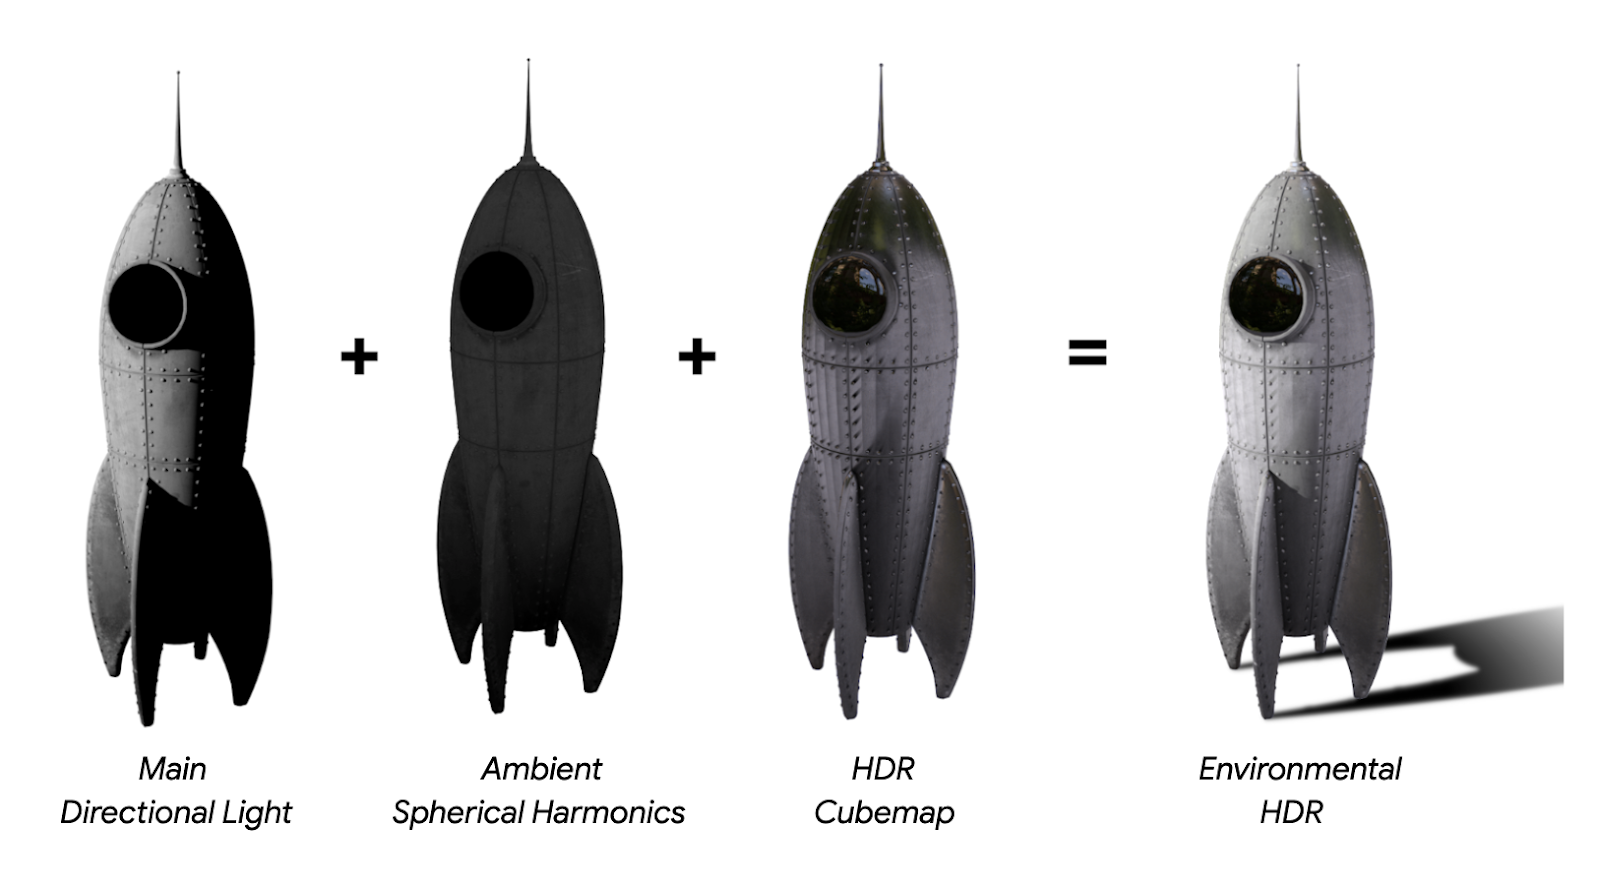
\includegraphics[width=\linewidth]{img/anwendung/arcore/arcore-light-estimation-environmentalhdr.png}
    \caption[Die Beleuchtungseinschaften und das kombinierte Endergebnis des Environmental HDR Modus.]{Die Beleuchtungseinschaften und das kombinierte Endergebnis des Environmental HDR Modus\protect\footnotemark.}
    \label{fig:anwendung-arcore-environmental-hdr}
\end{figure}
\footnotetext{Quelle Bild: https://developers.googleblog.com/2019/05/ARCore-IO19.html, zuletzt aufgerufen am 16.08.2022}

In dieser Arbeit wird dieser Modus verwendet, um die Reflektionen der Umgebung zu implementieren. Es werden in Kapitel \ref*{technische-umsetzung-licht} eigene Cubemaps aus Panoramabildern des SABA Gebäudes erstellt und benutzt. Dies ermöglicht das manuelle Einstellen der Wetterbedingungen. Damit wird in Kapitel \ref*{technische-umsetzung-wetterbedingungen} auch die Veränderung der Cubemaps sichtbar. 

Nachteil dabei ist, dass nur Cubemaps des SABA-Geländes genutzt werden. Da das SABA und Lyautey Gelände zum Zeitpunkt dieser Arbeit bebaut wird, verändert sich die Umgebung. Eine Erstellung von Cubemaps für jedes Gebäude würde sich demnach nicht lohnen, da sich der Ort verändert. Für eine weiterführende Arbeit wird daher empfohlen den Environmental HDR Mode zu verwenden. Die Cubemaps für die Reflektionen und das Environmental Lighting wird sich dann an den realen Gegebenheiten anpassen.

\subsubsection{User Interaction}
\label{technische-umsetzung-arcore-user-interaction}
Um Interaktionen des Nutzers zu den virtuellen Objekten zu implementieren, wird \textit{hit-testing} durchgeführt. In AR Foundation bzw. Unity wird dies \textit{Raycast} genannt. Daher wird diese Funktion nicht mit ARCore, sondern mit Unity implementiert. Das Prinzip ist gleich. Beim hit-testing wird ein virtueller Strahl vom Smartphone aus in die Umgebung erzeugt. Es werden Schnittpunkte zwischen diesen Strahl und virtuellen Objekten gefunden. Das \textit{Hit-Ergebnis} beinhaltet drei Informationen:

\begin{itemize}
    \item die Distanz des Smartphones zum Objekt, 
    \item die Position und die Orientierung des hits im Weltkoordinatensystem,
    \item die 3D Gemoetrie des getroffenen Objekts.
\end{itemize}

\begin{figure}[h]
    \centering
    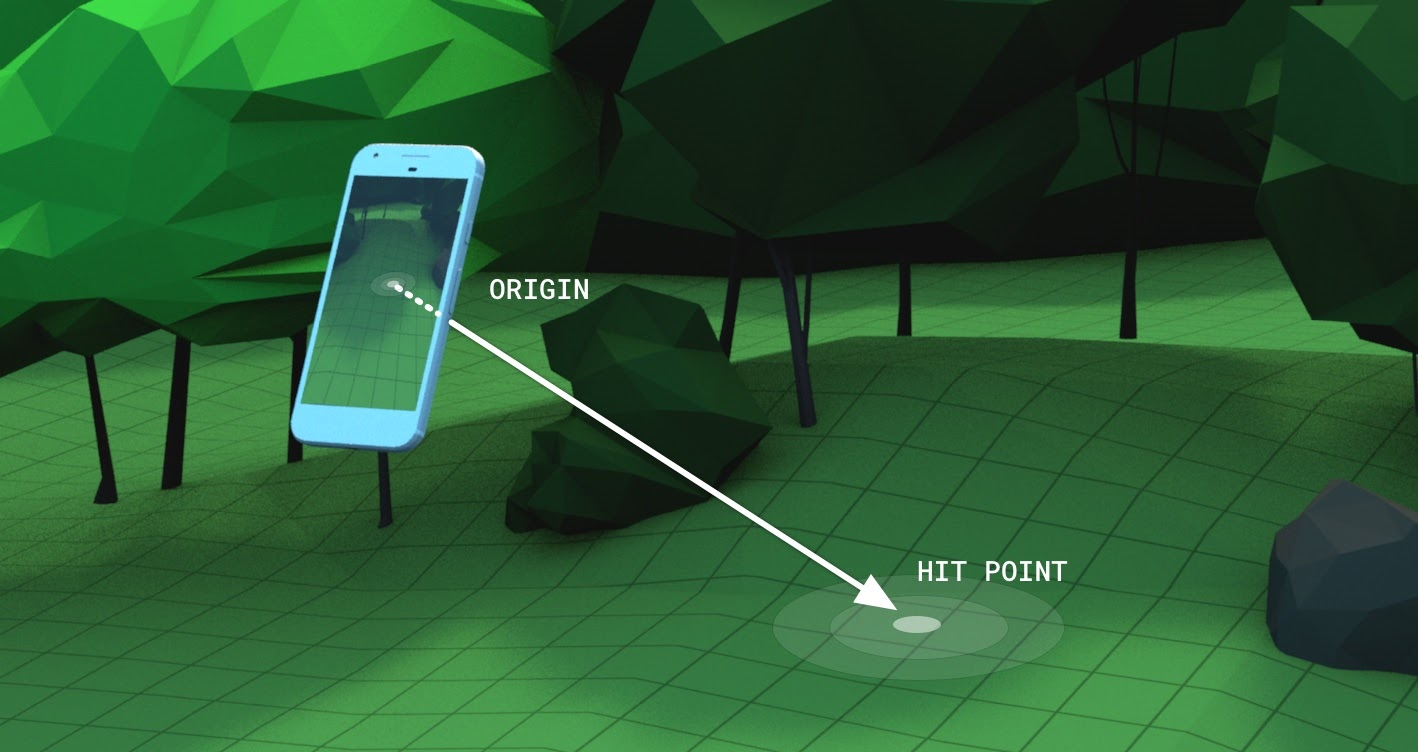
\includegraphics[width=8cm]{img/anwendung/arcore/hit-test-explainer.jpeg}
    \caption[Der hit-testing Strahl vom Smartphone trifft auf eine virtuelle Fläche und gibt ein Hit Ergebnis zurück.]{Der hit-testing Strahl vom Smartphone trifft auf eine virtuelle Fläche und gibt ein Hit Ergebnis zurück.\protect\footnotemark}
    \label{fig:anwendung-arcore-hit-test}
\end{figure}
\footnotetext{Quelle Bild: https://developers.google.com/ar/develop/hit-test, zuletzt aufgerufen am 09.08.2022}

In dieser Anwendung wird hit-testing dafür verwendet die Modelle auf den Flächen zu platzieren. Wird ein Hit zurückgegeben, wird dem Nutzer ein Pfeil auf der jeweiligen Fläche angezeigt. Der Pfeil dient als \textit{Placement Indicator}. Es hilft dem Nutzer bei der Platzierung der Objekte. Tippt der Nutzer auf den Bildschirm, wird das Gebäude an der Position des Hits platziert. Außerdem wird das hit-testing dazu genutzt bereits platzierte Gebäude zu detektieren. Die Implementierung in dieser Anwendug wird in Kapitel \ref*{technische-umsetzung-platzierung-auf-einer-beliebigen-flaeche-controller} erläutert. 

\subsubsection{Depth API}
\label{technische-umsetzung-arcore-depth-api}
Die Depth API generiert Tiefenbilder (\textit{depth maps}) um Tiefeninformationen der Umgebung zu erhalten. Es basiert auf der Arbeit von Flynn et al.\cite*{flynn2019}. Mit den Tiefenbildern werden die Position und die Größe von Objekten besser erkannt. Dies wird z.B. dafür genutzt, um \textit{Verdeckung (engl. Occlusion)} umzusetzen. Occlusion wird dann eingesetzt, wenn reale Objekte, die Näher am Betrachter liegen, das virtuelle Objekt verdecken. Wie in Abbildung \ref*{fig:anwendung-arcore-depth-api-occlusion} zu sehen wird die Katze vom realen Objekt verdeckt. Die Glaubwürdigkeit, dass eine echte Katze im Bild ist, steigt.

\begin{figure}[h]
    \centering
    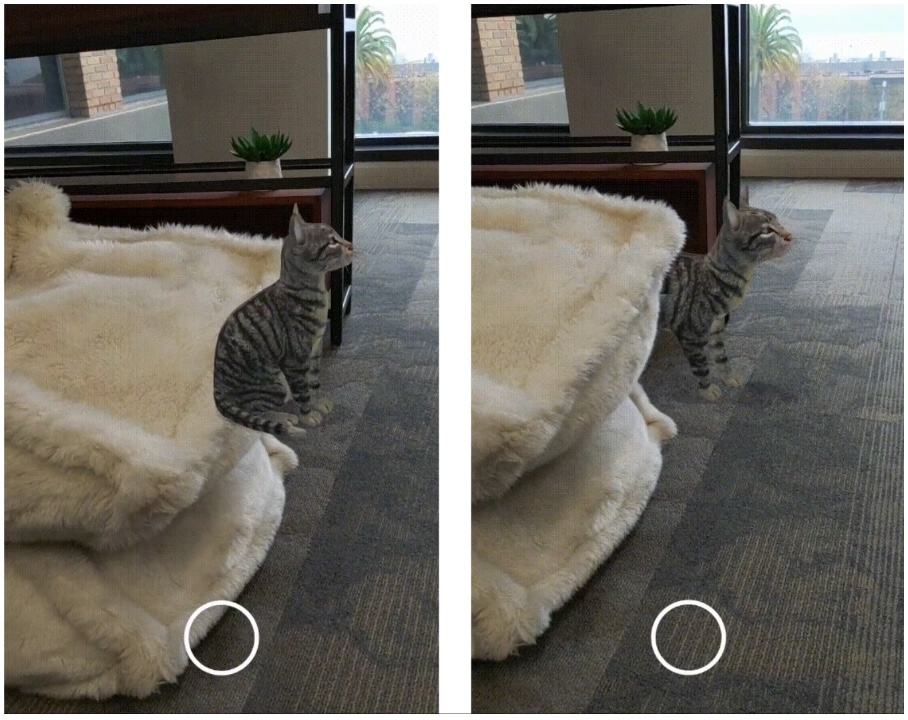
\includegraphics[width=8cm]{img/anwendung/arcore/arcore-depth-api-occlusion.jpg}
    \caption[AR ohne Occlusion (l.) und mit Occlusion (r.). Die virtuelle Katze wird durch das Objekt verdeckt.]{AR ohne Occlusion (l.) und mit Occlusion (r.). Die virtuelle Katze wird durch das Objekt verdeckt.\protect\footnotemark}
    \label{fig:anwendung-arcore-depth-api-occlusion}
\end{figure}
\footnotetext{Quelle Bild: https://developers.google.com/ar/develop/depth, zuletzt aufgerufen am 13.08.2022}

ARCore bietet zwei Ausgabemöglichkeiten für das Tiefenbild:

\begin{itemize}
    \item Raw Depth API liefert ein Tiefenbild mit hoher Genauigkeit. Dabei kann es vorkommen, dass nicht alle Pixel im Bild auch ein Tiefenwert erhält. Zusätzlich wird ein Konfidenzbild erzeugt.
    \item Full Depth API liefert ein geglättetes Tiefenbild. Pixel, die keinen Tiefenwert haben, erhalten einen geschätzten Wert.
\end{itemize}

Ein Konfidenzbild gibt jedem Pixel mit einem Tiefenwert einen Konfidenzwert zwischen 0 und 1. Je höher dieser Wert, desto höher ist die Wahrscheinlichkeit, dass die Tiefeninformation korrekt ist. Im Konfidenzbild wird dies durch die Pixelhelligkeit dargestellt. Je heller der Pixel im Konfidenzbild ist, desto höher ist der Konfidenzwert. Diese Funktion ist nützlich, um mit einem Threshold ungenaue Tiefeninformation auszuschließen.

Die Occlusion der Depth API zeigt in dieser Anwendung Probleme. Diese werden in Kapitel \ref*{probleme-grenzen-depth-api} aufgezeigt. Für den Anwendungszweck dieser Arbeit wird Occlsuion nur zum Testen für Entwickler in die Anwendung implementiert, da Ungenauigkeiten und Artefakte die Nutzererfahrung negativ beeinflussen.
%Neu in AR Core: global-scale location based Geospatial API